\clearpage{}
\section{Discuss tactics to achieve modifiability, performance, security,
reliability, robustness, usability.}

\subsection{Modifiability}

$\rightarrow$ Design must be easy to change. \newline

The goal is to minimize the number of software units requiring changes. This affects units in
two ways:

\begin{itemize}
    \item Directly affected: responsibilities change
    \item Indirectly affected: only implementation changes
\end{itemize}

\subsubsection{Tactics for directly affected units}

Cluster the anticipated changes.

\begin{itemize}
    \item Anticipate expected changes: encapsulate each anticipated change in one unit
    \item Cohesion: all pieces, data, and functionality of each unit contribute to its purpose
and responsibilities
    \item Generality: accommodate change by modifying a unit's inputs rather than modifying
the unit itself
\end{itemize}

\subsubsection{Tactics for indirectly affected units}

Reduce dependencies.

\begin{itemize}
    \item Coupling: reduce the degree to which a unit depends on another
    \item Interfaces: interact with other units only through their specified interface
    \item Multiple interfaces: provide a new interface for new data or services (preserving
existing interfaces)
\end{itemize}

\subsection{Performance}

$\rightarrow$ Constraints on system speed and capacity (response time, throughput, load).

\subsubsection{Tactics for immunity (preventing an attack)}

\begin{itemize}
    \item Ensure that all security features are included
    \item Minimize exploitable security weaknesses
\end{itemize}

\subsubsection{Tactics for resilience (recovering from an attack)}

\begin{itemize}
    \item Segment the functionality to contain attack
    \item Enable the system to quickly restore functionality
\end{itemize}

\subsection{Reliability}

$\rightarrow$ Performing correctly under assumed conditions. System correct = 100\% reliable.

\begin{figure}[!ht]
    \centering
    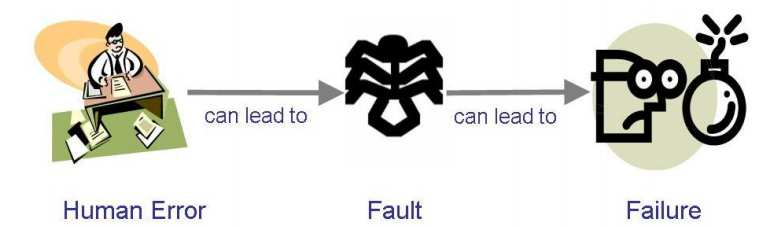
\includegraphics[width=\linewidth]{reliability.png}
    \caption{Reliability}
\end{figure}

Fault = a defect in a product

Two kinds of tactics:

\begin{itemize}
    \item Preventing faults, by writing well the code and avoiding human error.
    \item Tolerating faults, FDIR -> Fault detection, identification and recovery. Two kind of detection, active (look for symptoms) vs.\ passive wait fault.
\end{itemize}

\subsection{Robustness}

$\rightarrow$ Performing correctly under adverse conditions.

Safe = free from unacceptable behaviours.

Defensive design: anticipate external problems

Mutual suspicion: check inputs for correctness, consistency, pre-conditions

Redundant calculations (ex: space shuttle, radiation glitch)
State recovery tactics (same as for reliability)

\subsection{Recovery tactics}

Both robustness and reliability can use the following technics to recover from undesirable
state:

\begin{itemize}
    \item Undoing transaction (ex: database)
    \item Checkpoint / rollback (saved state)
    \item Backup
    \item Degraded service (provide an older stable version)
    \item Correct and continue (fix the symptoms)
    \item Report (returns to previous state and record the problem)
\end{itemize}

\subsection{Usability}
$\rightarrow$ Ease of use of the system.

Tactics at architectural level:
\begin{itemize}
    \item UI should be in its own software unit/layer
    \item Need a UI event handler process
    \item Support for UI functionality cancel/undo, views,\ldots
    \item Maintain a model of its environment Mme, industrial process
\end{itemize}
